\documentclass{beamer}

\usepackage[utf8x]{inputenc}
%\usetheme{Frankfurt}
%\usetheme{Ilmenau}
%\usetheme{Luebeck}
\usetheme{Madrid}
%\usetheme{Warsaw}

\title[Identificaci\'on de Letras Utilizando Bubbles]{Detecci\'on de Rasgos en la Identificaci\'on de Letras Utilizando Bubbles}
\subtitle{Intr. a Neurociencia Cognitiva y Computacional}
\author[Mart\'inez Soler,\\G\'omez Mayol,\\Cossio Mercado]{Christian Cossio Mercado,\\Mail\'en G\'omez Mayol,\\Miguel Mart\'inez Soler}
\institute{Departamento de Computaci\'on - FCEyN, UBA}
\date{31 de mayo de 2011}


\begin{document}

\begin{frame}
\titlepage
\end{frame}

\section{Introducci\'on}
  \subsection{Demostraci\'on}

      %estímulo máscara random
      \begin{frame}
      \begin{figure}
	
\includegraphics[scale=.2]{graficos/letra.png}
      \end{figure}
      \end{frame}

  %objetivos e hipótesis
  \subsection{Objetivos e Hip\'otesis}
      \begin{frame}
	\frametitle{Objetivos del experimento}
	\begin{itemize}
		\item Identificar rasgos utilizados por una persona para reconocer letras de distintas tipograf\'ias  \ldots 
      \end{itemize}

      \begin{block}{Hip\'otesis}
      \begin{itemize}
		\item El uso de tipograf\'ias ampliamente conocidas facilita el reconocimiento de letras 
		\item La eficiencia en el reconocimiento de las letras es inversamente proporcional a su complejidad 
		\item Los rasgos de cada letra var\'ian de acuerdo a la tipograf\'ia que se est\'e utilizando 
		\item Un observador ideal utilizar\'a rasgos distintos a los que utiliza una persona para identificar letras	
	  \end{itemize}
      \end{block}

      \end{frame}

  \subsection{Antecedentes}
  %Pelli
	\begin{frame}
	\frametitle{Feature Detection and Letter Identification(Pelli et al., 2006)}
	\begin{columns}[t]
	\column{.5\textwidth}
	\title{Feature Detection and Letter Identification (Pelli et al., 2006)}
	\begin{itemize}
		\item Cookbook de cualquier experimento de reconocimiento de Letras
		\item Concepto de complejidad (Attneave) FORMULA!
		\item Relación eficiencia/complejidad
	\end{itemize}

	\column{.5\textwidth}

	\begin{figure}
	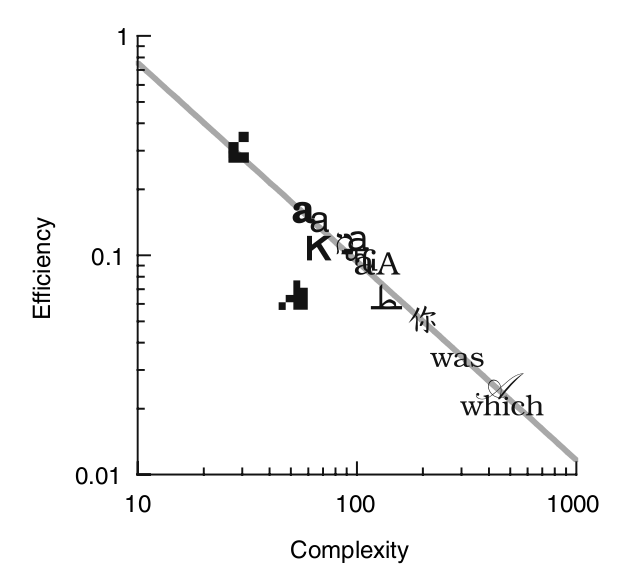
\includegraphics[width=\textwidth]{graficos/pelli4.png}
	\caption{Gráfico de eficiencia vs complejidad de varias tipografías distintas}
	\end{figure}

	\end{columns}
	\end{frame}

%Gosselin
	\begin{frame}
	\frametitle{Bubbles: a technique to reveal the use of information in recognition task (Gosselin \& Schyns, 2001)}
	\begin{columns}[t]
	  \column{.5\textwidth}
	  
	    \begin{itemize}
	    \item Cookbook de cualquier experimento con Bubbles
	    \item Bubbles locas
	    \item AGREGAR IMAGEN DE BUBBLES (MASCARA)
	    \end{itemize}
	  
	  \column{.5\textwidth}
	  \begin{figure}
	  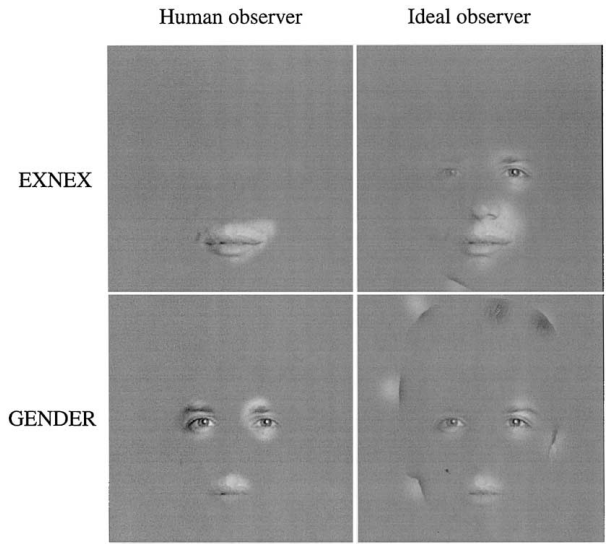
\includegraphics[width=\textwidth]{graficos/gosselin2.png}
	\caption{Bubbles aplicada al reconocimiento de expresión (ENEX) y género (GENDER)}
	  \end{figure}
	  \end{columns}
	\end{frame}


	%Fiset
	\begin{frame}
	\frametitle{Feature for Identification of Uppercase and Lowercase Letters (Fiset et al., 2008)}

	\begin{columns}[t]
	\column{.5\textwidth}
	  \begin{figure}
	    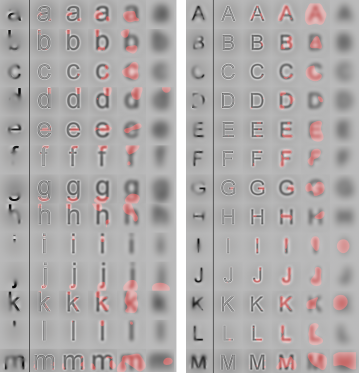
\includegraphics[width=.6\textwidth]{graficos/fiset1.png}
	\caption[Fiset et al]{Clasificación de imágenes por observadores humanos}
	  \end{figure}
	  \column{.5\textwidth}
	  \begin{figure}
	    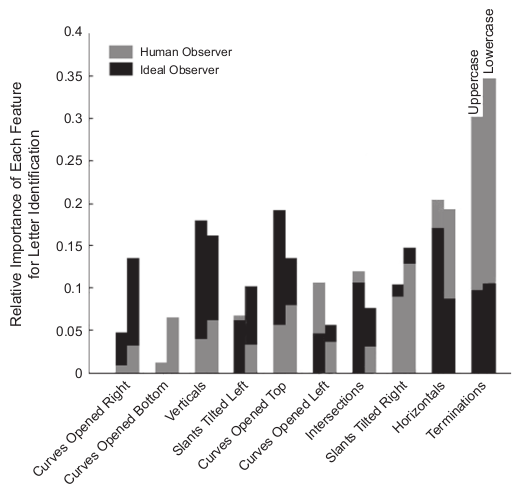
\includegraphics[width=\textwidth]{graficos/fiset5.png}
	\caption{Uso relativo de 10 rasgos de letras para el reconocimiento de letras Arial}
	  \end{figure}
	\end{columns}

	\end{frame}


\section{Experimento}
  \subsection{Dise\~no}

	%Elección tipografías
	\begin{frame}
	\frametitle{Elecci\'on de tipograf\'ias}
	\begin{figure}
	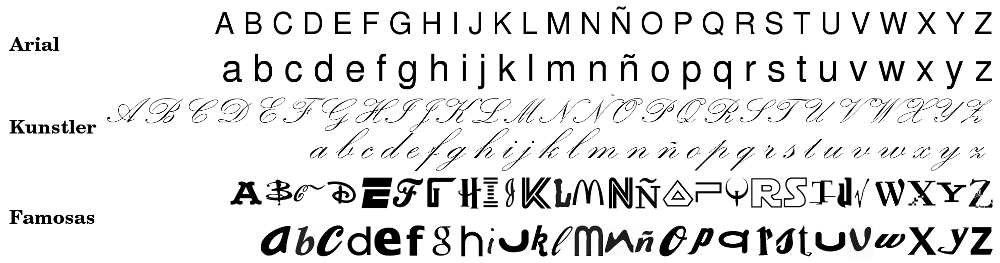
\includegraphics[width=\textwidth]{graficos/letras.png}
	\caption{tipograf\'ias elegidas}
	\end{figure}
	Boxplot de complejidades
	\end{frame}

	%estímulos
	\begin{frame}
	\frametitle{Est\'imulos}
	\begin{figure}
	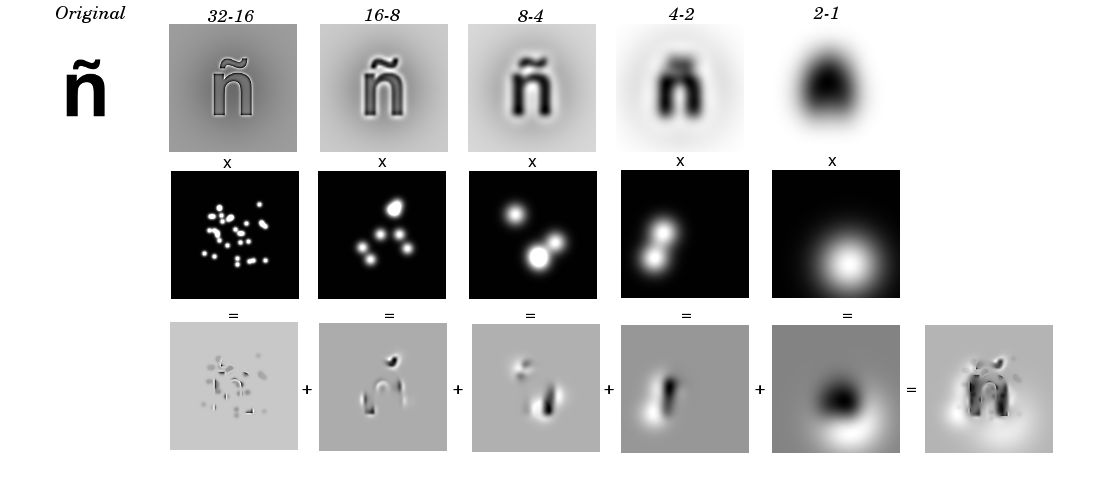
\includegraphics[width=\textwidth]{graficos/estimulofinal.png}
	\caption{Armado del est\'imulo final}
	\end{figure}
	\end{frame}

	%Jueves
	\begin{frame}
	\frametitle{Primeros Pasos. Jueves 12/5}
	\begin{itemize}
	\item 13 sujetos
	\item Pocos bloques
	\item Muchas burbujas
	\item Muy poca información \pause
	\item Muchos gastos en golosinas\pause
	\end{itemize}
	\textbf{Solución}: Ampliar set de datos y ajustar parámetros (bloques y burbujas)
	\end{frame}

	%Recauchutaje
	\begin{frame}
	\frametitle{Rediseño}
	\begin{itemize}
	\item Correcciones de errores menores (randoms, cantidad de burbujas (no se mostraba en todas las bandas), etc.)
	\item Más bloques por sujeto, por lo tanto, experimento más largo
	\item Mejora en la cantidad de burbujas inicial (mayor complejidad, mayor cantidad de burbujas iniciales)
	\item Filtrando casos en que no se llegó al 52\%
	\end{itemize}

	\end{frame}


	%Final
	\begin{frame}
	\frametitle{Etapa Final}
	\begin{itemize}
	\item 6 sujetos
	\item edades entre 21-33 años
	\item con estudios superiores
	\item se les mostraron alrededor de 2000 est\'imulos
	\item \underline{experimentadores sujetos}... 2500 est\'imulos
	\end{itemize}
	\end{frame}


  \section{Resultados}

	%RASGOS
	\begin{frame}
	\frametitle{Cálculo de Rasgos}
	\begin{columns} [t]
	\column{.5\textwidth}
	\begin{figure}
	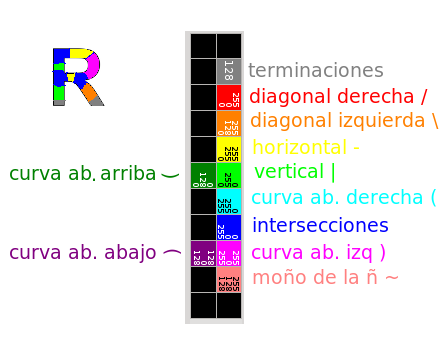
\includegraphics[width=.8\textwidth]{graficos/REFERENCIA.png}
	\caption{Código de colores para poder identificar los rasgos automáticamente}
	\end{figure}
	\column{.5\textwidth}
	\begin{figure}
	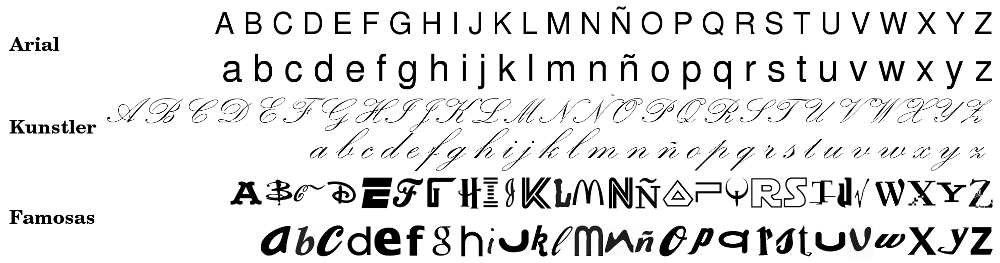
\includegraphics[width=.5\textwidth]{graficos/letras.png}
	\caption{Uso relativo de los rasgos necesarios para identificar letras}
	\end{figure}
	\end{columns}
	\end{frame}



%Discusión
\section{Lecciones Aprendidas}
	\begin{frame}
	\frametitle{Lecciones Aprendidas}
	\begin{itemize}
	\item Cantidad de respuestas necesarias (o estímulos a mostrar): 156.000= 3.9 días de experimentación continua.
	\item Resulta una técnica útil para el muestreo de espacios de un estímulo determinado
	\end{itemize}
	\end{frame}

	\begin{frame}
	\frametitle{Trabajos Futuros}
	\begin{itemize}
	\item Bubbles en habla
	\end{itemize}
	\end{frame}


\author[Cossio Mercado,G\'omez Mayol,Mart\'inez Soler]{Mail\'en G\'omez Mayol,\\Miguel Mart\'inez Soler,\\Christian Cossio Mercado}
\begin{frame}
 \titlepage
\end{frame}


\end{document}
